\chapter{Energy measurement tools and techniques}


The most recent scientific applications have to process and store
a considerable volume of data. It is foreseeable that the volume of
data will increase considerably in the future, as technology and
requirements enhance. In addition to the physical limitations in
terms of power density, this phenomenon also increase considerably
the costs with energy in a HTC system. Thus, energy consumption has
become a major concern amongst the scientific community.



\textbf{re-write and re-organize everything from now on}

In order to find and develop better solutions for improving energy
efficiency in High Energy Physics (HEP) computing, it is important to understand
how energy is used by the HEP systems themselves. We describe several
tools and techniques that facilitate researchers to reach that goal.

As energy efficiency becomes a concern, new solutions have been
considered to develop energy efficient systems. One potential
solution is to replace the traditional Intel x86 architectures by
low power architectures such as ARM. A comparison of the energy
efficiency between ARMv7 and x86 Intel architecture is conducted
in this article. The experiments use CMS workloads and rely on the
techniques and tools described earlier to perform the measurements.


\section{Tools and techniques for energy measurement}

When optimizing power usage, there are two granularities at which
one can look at a computing system. The coarser granularity
takes into account the behavior of the whole node (or
some of its passive parts, e.g.\ the transformer) as part of a rack
in a datacenter. This is usually investigated when
engineering and optimizing computing centers. Alternatively,
a more detailed approach is to
look into the components which make up the active parts of a
node, in particular the CPU and its memory subsystem since these
are responsible for a sizeable fraction of the consumed power.
They are also the place where the largest gains in terms of efficiency 
can be obtained through optimizations in the software.

If one is simply interested in the coarse power consumption by node,
external probing devices can be used: monitoring interfaces
of the rack power distribution units, plugin meters and non-invasive
clamp meters (allowing measurement of the
current pulled by the system by induction without making physical
contact with it). They differ mostly in terms of flexibility.
Their accuracy is typically a few percent for power, whereas their time
resolution is in the order of seconds. This is more than enough
to optimize electrical layout of the datacenters or to provide a
baseline for more detailed studies.

A alternative approach takes into account the internal structure of a
computing element of an HTC system, as shown in figure 
~\ref{fig:power-consumption-model}. Nowadays, every board manufacturer
provides on-board chips which monitor energy consumption of
different components of the system. These
allow energy measurements of fine grained detail, as it is possible
to individually monitor energy consumption of components such as
the CPU, its memory subsystem, and others. An example of this chip
monitors is the Texas Instruments TI INA231~\cite{TIINA231} current-churn
and power monitor which is found on the ARMv7 developer board which
we used for our studies. It is quite common in the industry.
Compared to external methods, these on-board components provide
high accuracy and reasonably high precision measurements (millisecond
level).

\begin{figure}[tbp]
\centering
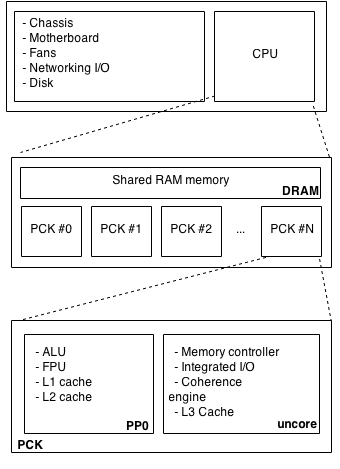
\includegraphics[width=50mm]{img/energy_model.png}
\caption{Components that contribute for power consumption in HPC}
\label{fig:power-consumption-model}
\end{figure}

A special and slightly different case of these on-board monitors
is a new technology called Running Average Power Limit (RAPL),
provided by Intel beginning from the Sandy Bridge family of processors.

Contrary to other solutions, which are implemented as discrete
chips, RAPL is embedded as part of the CPU package itself and
provides information on the CPUs own subsystems. In particular RAPL
provides data for three different domains: \textbf{package} (pck),
which measures energy consumed by the system's sockets, \textbf{power
plane 0} (pp0), which measures energy consumed by the CPU core(s),
and \textbf{dram}, which accounts for the sum of energy consumed
by memory in a given socket, therefore excluding the on-core
caches~\cite{INTELMAN}. As for the discrete components case, the
timing resolution of measurements is in the millisecond range~\cite{RAPL1}.
This is fine enough to permit exploiting such data to build an energy
consumption sampling profiler for applications, similar to how performance
sampling profilers work (see section~\ref{sec:sampling}).
Finally, in addition to power
monitoring of the sockets, RAPL can limit the power consumed by the
different domains. This feature, usually referred as power capping,
allows the user to define the average power consumption limit of a
domain in a defined time window and allows more accurate independent
measurements of the non limited components.




\section{Power efficiency measurements with x86-64 and ARMv7}

In this section, we demonstrate the potential of some of the
tools we previously described. To that end, we perform
several measurements of workloads from CERN, running on different
architectures. The workloads used in the experiment run on top of
Intel x86-64 architecture, traditionally used in HTC and data centers
and 32 bit ARMv7 architectures (for similar studies for 64bit ARMv8
and Xeon Phi, please refer to~\cite{ABD2014}). The ARM architecture,
initially developed for mobile devices, has been
considered~\cite{ACAT13ARM, CHEP13ARMPHI} as a potential alternative
to Intel in HTC, given its energy efficient computing. We also
present a brief comparison between ARM and Intel architectures from
the energy consumption perspective, based on the results obtained.

\subsection{Tools and techniques}

For the Intel architecture, we used the RAPL technology to perform measurements
of the energy consumed by the package, DRAM and cores 
(figure~\ref{fig:power-consumption-model}).
The external measurements for the baseline were performed using a
rack PDU, which provides an online API to gather the energy consumed
by the system on the rack at a sampling rate of 1 second.
For the ARM board, we used the Texas Instrument power monitor
chip TI INA231 which allows reading of the energy consumed by the
cores and dram at a sampling rate of microseconds. The chip was
embedded in the board from the vendor. For the external measurements,
we used an external plug-in power monitor with a computer interface
for gathering and storing the results.
In both cases we read the data as it was exposed to the system via
the sysfs / devfs knobs.
